\documentclass[11pt,a4paper]{article}
\usepackage{amsmath}
\usepackage{amssymb}
\usepackage{graphicx}
\usepackage{verbatim}
\begin{document}
	\noindent
	Martin Lundfall, Henri Bunting, Malte Siemers, Patrik Bey
	\begin{centering}
		\section*{Exercise sheet 12 - Machine Intelligence I}
	\end{centering}
	\subsection*{12.1 - Implementation of belief propagation}
\subsubsection*{a)}
The directed acyclic graph of the network is the previously illustrated figure below.
	\begin{figure}[h]
		\caption{DAG illustrating joint probability distribution}
		\centering
		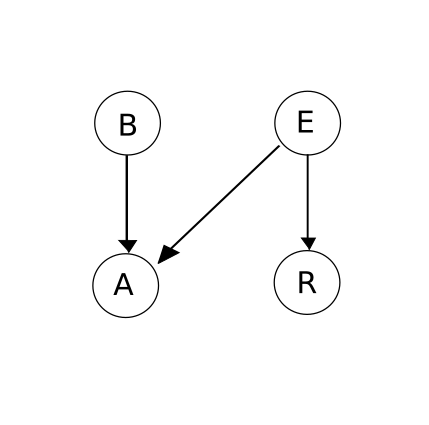
\includegraphics[width=.5\textwidth]{graph}
	\end{figure}
\subsubsection*{b)}
First, we construct the moral graph of DAG above.
	\begin{figure}[h]
		\caption{Moral graph of the network}
		\centering
		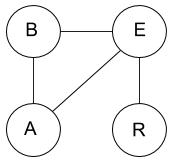
\includegraphics[width=.3\textwidth]{MORAL}
	\end{figure}
\newpage
To construct the junction tree, we compress cliques to single nodes. The node C1 is clique of $\{A, B, E\}$ in the moral graph above and the node C2 is the clique $\{E, R\}$ and the link is the separator $E$. The clique potential at C1 is the product:
\begin{equation*}
\begin{split}
P(E)P(B)P(A|B,E)=\\
P(E)P(B)\sum_{e \in E, b \in B}(P(A|e, b)\\
=0.000001\cdot 0.01\cdot\\
(0.001\cdot0.99\cdot0.99999+0.41\cdot0.99\cdot0.000001+\\
0.95\cdot0.01\cdot0.99999+0.98\cdot0.01\cdot0.000001) = 1.049^{-10}
\end{split}
\end{equation*}
The separator potential is initialized to 1. The clique potential of C2 is: $P(E)P(R|E)=P(E)=0.000001$
\begin{figure}[h]
	\caption{Junction tree of the network}
	\centering
	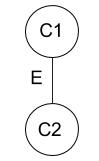
\includegraphics[width=.2\textwidth]{junction}
\end{figure}
\subsubsection*{c)}
The following marginals were calculated with the bayesian package for python we also used in assignment 11:
	\begin{verbatim}
	+----------------+-------+----------+
	| Node           | Value | Marginal |
	+----------------+-------+----------+
	| alarm          | False | 0.989510 |
	| alarm          | True  | 0.010490 |
	| burglary       | False | 0.990000 |
	| burglary       | True  | 0.010000 |
	| earthquake     | False | 0.999999 |
	| earthquake     | True  | 0.000001 |
	| radioBroadcast | False | 0.999999 |
	| radioBroadcast | True  | 0.000001 |
	+----------------+-------+----------+
	\end{verbatim}
\subsection*{d)}
The probability that a burglary has happend when the alarm turns on is
\begin{equation*}
\begin{split}
  P(B=t|A=t) = \frac{P(A=t|B=t)P(B=t)}{P(A=t)}=\\
  \frac{(P(A=t|B=t,E=t)P(E=t)+P(A=t|B=t,E=f)P(E=f))P(B=t)}{P(A=t)}=\\
  \frac{(0.98*10^{-6}+0.95*0.999999)*0.01}{0.010490}=0.905624...
  \end{split}
\end{equation*}
The influence of hearing the radio while an alarm goes off is the following:
\begin{equation*}
  \begin{split}
  P(B=t|A=t,E=t)  = \frac{P(E=t, A=t | B=t)P(B=t)}{P(A=t,E=t)}= \\
  \\
  =  \frac{P(A=t |E=t, B=t)P(B=t)P(E=t)}{P(A=t|E=t)P(E=t)}= \\
  \\
  =  \frac{P(A=t| B=t, E=t)P(B=t)}{P(A=t|B=t,E=t)P(B=t)+P(A=t|B=f,E=t)P(B=f)} \\
  = \frac{0.98*0.01}{0.98*0.01+0.41*0.99}=0.02357...
  \end{split}
\end{equation*}
The probability, that a burglary had happened when the alarm goes off while one heard about an earthquake in the radio is drastically smaller than without the information on the earthquake.

\subsection*{12.2 - Bayesian Inference}
  \subsection*{a}
Generative model\\
Generative models diverge from strict assignment of labels to allow for probabilistic assignment.  It represents a hypothesis about the causes.\\
We can say that some latent variable, for example y*, is the driving factor behind our label assignment function, y.\\
An example of a generative model is additive noise.  We can model our y as:\\
\begin{equation*}
y = y* + \eta
\end{equation*}
Here, y is modeled by the latent $y* + \eta$ for some noise function $\eta$ \\\\
Prior distribution\\
The prior distribution represents some initial beliefs of values for our parameters.  It is modeled by: $P(\theta)$\\\\
Likelihood function\\
$L(\theta)$\\
In Maximum Likelihood estimation, we take a subset of the observations and maximize this to give us a $\theta$ which we then use to make predictions for future features.  It is a product of the probabilities.\\\\
Posterior distribution\\
After observing data, we update our beliefs.\\
$(P(x1, ..., xn | \theta) * P(\theta)) / P(x1, ..., xn)$\\\\
Predictive distribution\\
How we can predict new data.\\
$P(x^{n+1} | x1, ..., xn) = \int (P(x^{n+1} | \theta) * P(\theta | x1, ... , xn)d\theta$\\
While this is a major advantage for Bayesians, it is also computationally expensive.\\

  \subsection*{b}
In the Bayesian approach, we update the knowledge base after every new piece of data, so we do not encounter the problem of over-/under-fitting.

\end{document}
